% Options for packages loaded elsewhere
\PassOptionsToPackage{unicode}{hyperref}
\PassOptionsToPackage{hyphens}{url}
%
\documentclass[
]{article}
\usepackage{amsmath,amssymb}
\usepackage{iftex}
\ifPDFTeX
  \usepackage[T1]{fontenc}
  \usepackage[utf8]{inputenc}
  \usepackage{textcomp} % provide euro and other symbols
\else % if luatex or xetex
  \usepackage{unicode-math} % this also loads fontspec
  \defaultfontfeatures{Scale=MatchLowercase}
  \defaultfontfeatures[\rmfamily]{Ligatures=TeX,Scale=1}
\fi
\usepackage{lmodern}
\ifPDFTeX\else
  % xetex/luatex font selection
\fi
% Use upquote if available, for straight quotes in verbatim environments
\IfFileExists{upquote.sty}{\usepackage{upquote}}{}
\IfFileExists{microtype.sty}{% use microtype if available
  \usepackage[]{microtype}
  \UseMicrotypeSet[protrusion]{basicmath} % disable protrusion for tt fonts
}{}
\makeatletter
\@ifundefined{KOMAClassName}{% if non-KOMA class
  \IfFileExists{parskip.sty}{%
    \usepackage{parskip}
  }{% else
    \setlength{\parindent}{0pt}
    \setlength{\parskip}{6pt plus 2pt minus 1pt}}
}{% if KOMA class
  \KOMAoptions{parskip=half}}
\makeatother
\usepackage{xcolor}
\usepackage[margin=1in]{geometry}
\usepackage{graphicx}
\makeatletter
\def\maxwidth{\ifdim\Gin@nat@width>\linewidth\linewidth\else\Gin@nat@width\fi}
\def\maxheight{\ifdim\Gin@nat@height>\textheight\textheight\else\Gin@nat@height\fi}
\makeatother
% Scale images if necessary, so that they will not overflow the page
% margins by default, and it is still possible to overwrite the defaults
% using explicit options in \includegraphics[width, height, ...]{}
\setkeys{Gin}{width=\maxwidth,height=\maxheight,keepaspectratio}
% Set default figure placement to htbp
\makeatletter
\def\fps@figure{htbp}
\makeatother
\setlength{\emergencystretch}{3em} % prevent overfull lines
\providecommand{\tightlist}{%
  \setlength{\itemsep}{0pt}\setlength{\parskip}{0pt}}
\setcounter{secnumdepth}{-\maxdimen} % remove section numbering
\usepackage{multicol}
\usepackage{natbib}
\usepackage{graphicx}
\usepackage{caption}
\ifLuaTeX
  \usepackage{selnolig}  % disable illegal ligatures
\fi
\IfFileExists{bookmark.sty}{\usepackage{bookmark}}{\usepackage{hyperref}}
\IfFileExists{xurl.sty}{\usepackage{xurl}}{} % add URL line breaks if available
\urlstyle{same}
\hypersetup{
  pdftitle={Linux Authentication and PAM},
  pdfauthor={Henry Roeth},
  hidelinks,
  pdfcreator={LaTeX via pandoc}}

\title{Linux Authentication and PAM}
\usepackage{etoolbox}
\makeatletter
\providecommand{\subtitle}[1]{% add subtitle to \maketitle
  \apptocmd{\@title}{\par {\large #1 \par}}{}{}
}
\makeatother
\subtitle{Face Recognition}
\author{Henry Roeth}
\date{2024-02-16}

\begin{document}
\maketitle
\begin{abstract}
In computer security, authentication is the process of confirming
someone is who they claim to be when attempting to access any kind of
computer system through the confirmation of something they have,
something they know, or something they are. It is important to always
maintain and improve the integrity of computer systems' authentication
schemes as new security threats arise. The Linux kernel invokes the
standard Unix authentication process across the majority of its
applications. However, as new forms of authentication are developed, it
is inefficient to individually reconfigure applications such that the
desired authentication scheme is incorporated. The PAM (Pluggable
Authentication Module) mechanism in Linux integrates various low-level
authentication schemes into a high-level API, allowing programs that
require some form of authentication to be developed independently from
the desired authentication scheme. This integrated research aims to
demonstrate the function and importance of PAM in Linux authentication
with the invocation of a face recognition PAM security module. Real-time
face detection and recognition is performed using the Haar Cascade
Classifier and the LBPH (Local Binary Patterns Histograms) feature-based
face recognition method.
\end{abstract}

\begin{multicols}{2}
\section{Introduction}
The \cite{viola2001rapid} Linux \cite{ahonen2004} kernel \cite{geisshirt2007} invokes the standard Unix authentication process across most of its applications (e.g., common-auth, sshd, su, and sudo). When developers are creating and updating applications, it would prove quite inefficient to individually reconfigure application logic such that it aligns with the newly desired authentication scheme. This would mean restructuring code and requiring other dependencies. With this in mind, developers need a way to invoke authentication schemes independently from applications, allowing for a more modular approach. This enables programs to run separately. Much like it's father kernel (Unix) the Linux kernel invokes these modular authentication schemes via the PAM (Pluggable Authentication Module) mechanism. One might think of this as a multitool. Just as a multitool can have different tools for various purposes like cutting, screwing, or opening, PAM provides different authentication methods for Linux. Depending on what you need to authenticate—be it through passwords, biometrics, or other means—you can plug in the appropriate tool/module into PAM to handle the authentication process effectively. This integrated research aims to display this function with the creation of a modular authentication scheme—face recognition.

\section{Overview of Linux Authentication}
Linux authentication involves several components. Centrally are the /etc/passwd and /etc/shadow files. In /etc/passwd, user account information such as usernames, user IDs, group IDs, and home directories are stored. The tangible passwords are more securely stored in /etc/shadow. It is here where there are hashed passwords and other security-related information. Each line in /etc/shadow represents a user account and includes uniquely populated fields like usernames, encrypted passwords, password aging and expiration details, and account lockout information. When any user attempts to login to the machine, the system hashes the entered password using the same algorithm as the one stored in /etc/shadow. If the hashed passwords match, access is granted to the user. More specifically, hashing involves the conversion of a password into a fixed-length string of characters using a cryptographic hash function. This process is irreversible, meaning the original password cannot be easily derived from the hash. Another additional measure of security that is implemented in the hashing process is salting. Salting is where a random value (a salt) is added to the password before hashing. This prevents attackers from using precomputed hash tables, also known as rainbow tables, to crack passwords. These unique fields in the /etc/shadow file are separated by colons, with each field serving a specific purpose. These fields may typically include the username, the hashed password, the last password date, the minimum and maximum password age, the password warning period, the password inactivity period, the account expiration date, and the account expiration date warning. To summarize, the integrity of the Linux authentication process relies on secure data storage of hashed passwords, salting for additional security, and an automated management system of user account information. As this relates to PAM, the invoked module (found in the directory /lib/*/security) is the primary logic to which the input password is hashed and compared to the corresponding hash in the /etc/shadow file; it is then followed by either a success or failure being return to the PAM mechanism.

\end{multicols}

\begin{figure}[htbp]
  \centering
  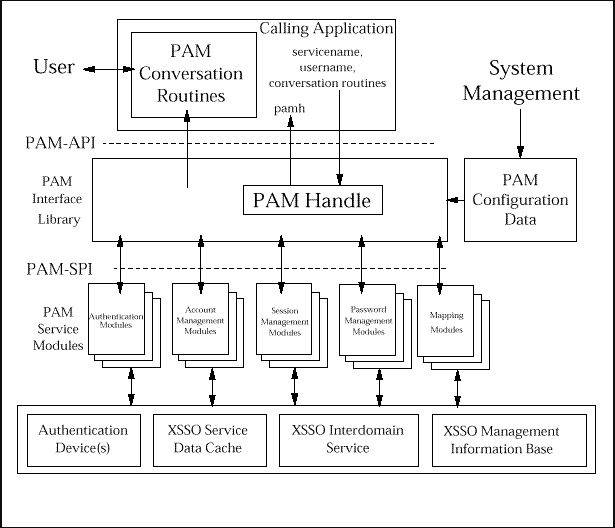
\includegraphics[width=0.4\linewidth]{pam_configuration.png}
  \caption{Example image 1 with a caption.}
\end{figure}

\begin{multicols}{2}
\section{PAM Configuration}
The PAM mechanism generally handles all authentication in Linux.  

\section{Authentication and Biometrics}
To be continued.

\end{multicols}

\bibliographystyle{apalike}
\bibliography{irc_1_ref.bib}

\end{document}
